\documentclass[12pt, a4paper]{article}
\usepackage{fontspec}
  \defaultfontfeatures{Mapping=tex-text}
  \setromanfont [Ligatures={Common}]{Linux Libertine O}
\usepackage{sectsty}
  \sectionfont{\upshape\Large}
  \subsectionfont{\upshape\large}
  \subsubsectionfont{\mdseries\scshape\normalsize}
\usepackage{tabularx}
\usepackage[usenames,dvipsnames,svgnames,table]{xcolor}
  \definecolor{tnzbrown}{HTML}{503E32}
  \definecolor{tnzgreen}{HTML}{118A47}
\PassOptionsToPackage{hyphens}{url}\usepackage{hyperref}
  \hypersetup{colorlinks=true,linkcolor=tnzgreen,urlcolor=tnzgreen}
\usepackage[font={color=tnzbrown}]{caption}
\usepackage{tocloft}
  \setlength\cftbeforesecskip{1pt}
\title{\textbf{How to... Fix HP printer “filter failed” error in (Ubuntu) Linux }}
\author{Joaquim Baeta}
\date{February 6, 2015\\ \normalsize \emph{(\textbf{Updated} \today)}}

\begin{document}
\maketitle

\tableofcontents
\vspace{1cm}

\section*{Error: ``filter failed"}\addcontentsline{toc}{section}{Error: ``filter failed"}

\noindent \emph{\textbf{Update, 2015-02-06:} As of a recent upgrade to Xubuntu 14.10, jumping straight to the third solution still fixes this error. It can also fix the ``cups filter failed", ``print service unavailable", and ``bad file descriptor" errors, according to an anonymous commenter.\footnote{\url{http://thenumberzero.blogspot.com/2014/02/how-to-fix-hp-printer-filter-failed.html?showComment=1424962297455\#c7199534845988630867}}}\\

\noindent My printer suffered a paper jam. After releasing the paper, I found that the printer was unwilling to print anything. The specific error was “filter failed”.

\subsection*{Diagnosing}\addcontentsline{toc}{subsection}{Diagnosing}

The first step is to open CUPS. In your browser's urlbar, type “localhost:631”. If at any point, CUPS asks for your password, enter it as you would in the terminal. To confirm this error, click on the \emph{Jobs} tab (Figure~\ref{fig1}). 

\begin{figure}[h]
  \centering
  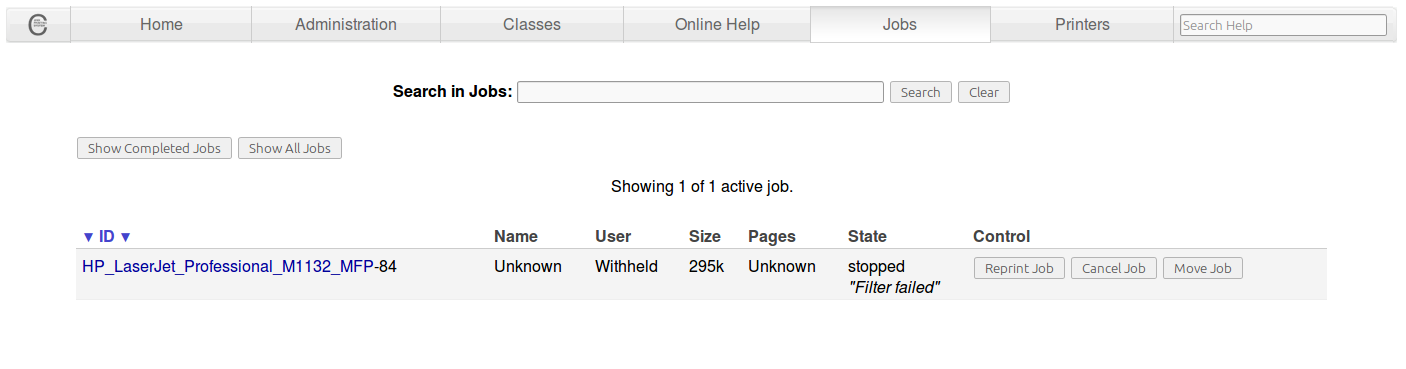
\includegraphics[width=1\textwidth]{imgs/filter-failed-1.png}
  \caption{Confirming the ``filter failed" error in CUPS.}
  \label{fig1}
\end{figure}

\noindent As you can see under \emph{State}, I'm getting the “filter failed” error.

\subsection*{Solution 1: re-install printer}\addcontentsline{toc}{subsection}{Solution 1: re-install printer}

Now click on the \emph{Printers} tab, and then click on your printer (Figure~\ref{fig2}).

\newpage
\begin{figure}[h]
  \centering
  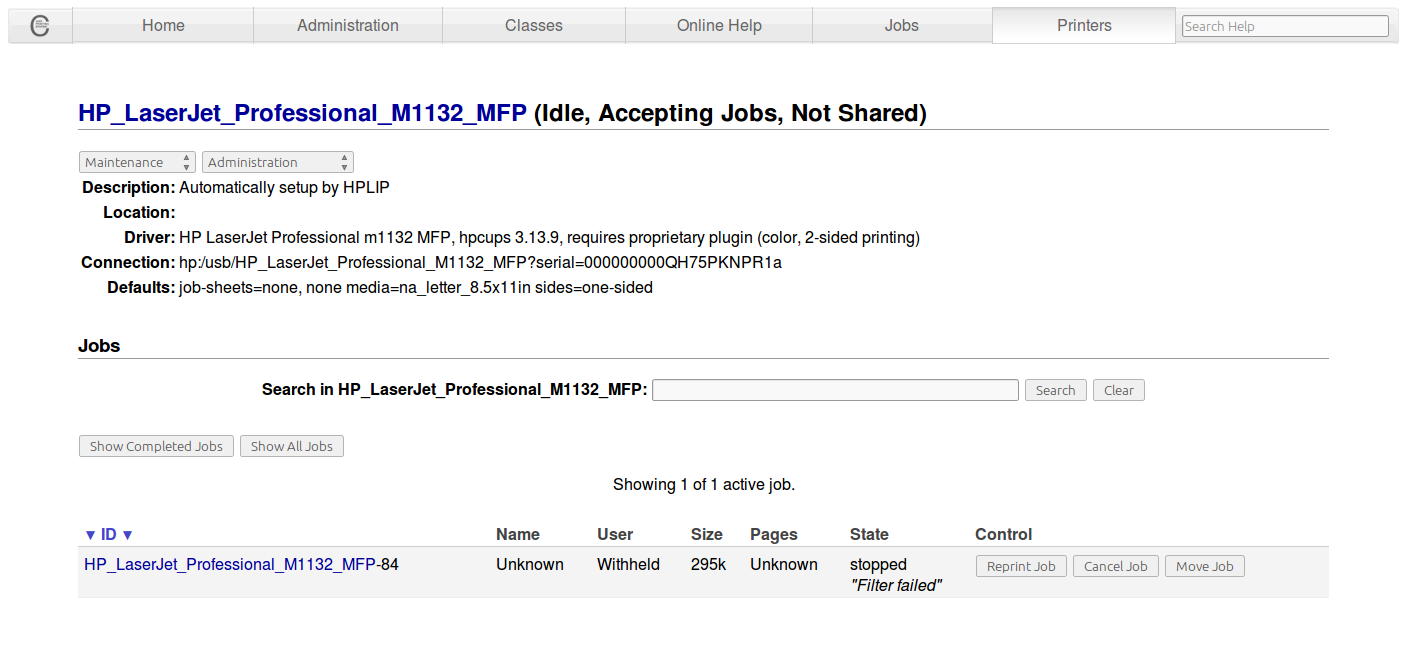
\includegraphics[width=1\textwidth]{imgs/filter-failed-2.png}
  \caption{HP\_LaserJet\_Professional\_M1132\_MFP page in CUPS.}
  \label{fig2}
\end{figure}

\noindent Under the \emph{Administration} menu, you will see an option to delete the printer (Figure~\ref{fig3}).

\begin{figure}[!h]
  \centering
  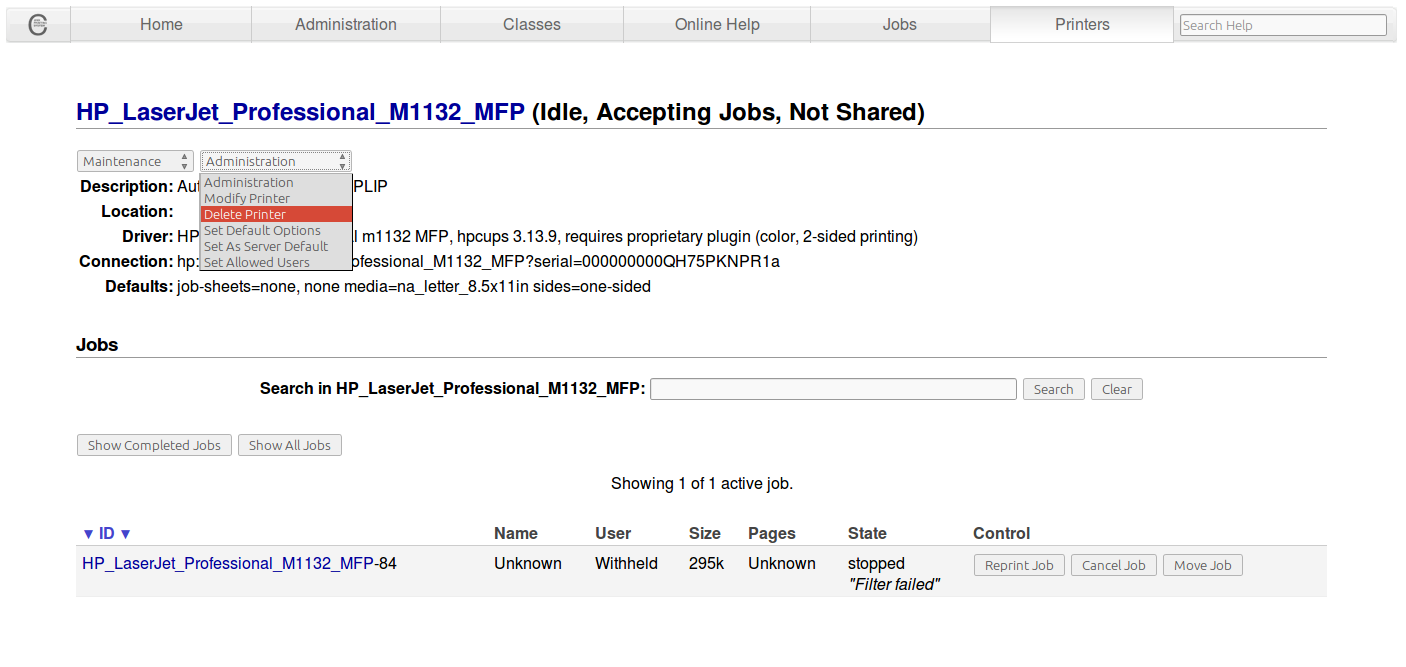
\includegraphics[width=1\textwidth]{imgs/filter-failed-3.png}
  \caption{Deleting the printer using the administration menu in the CUPS \emph{Printers} page.}
  \label{fig3}
\end{figure}

\noindent When asked to confirm, click \emph{Delete Printer}. In the \emph{Administration} tab, add the printer (Figure~\ref{fig4}). 

\newpage
\begin{figure}[!hbp]
  \centering
  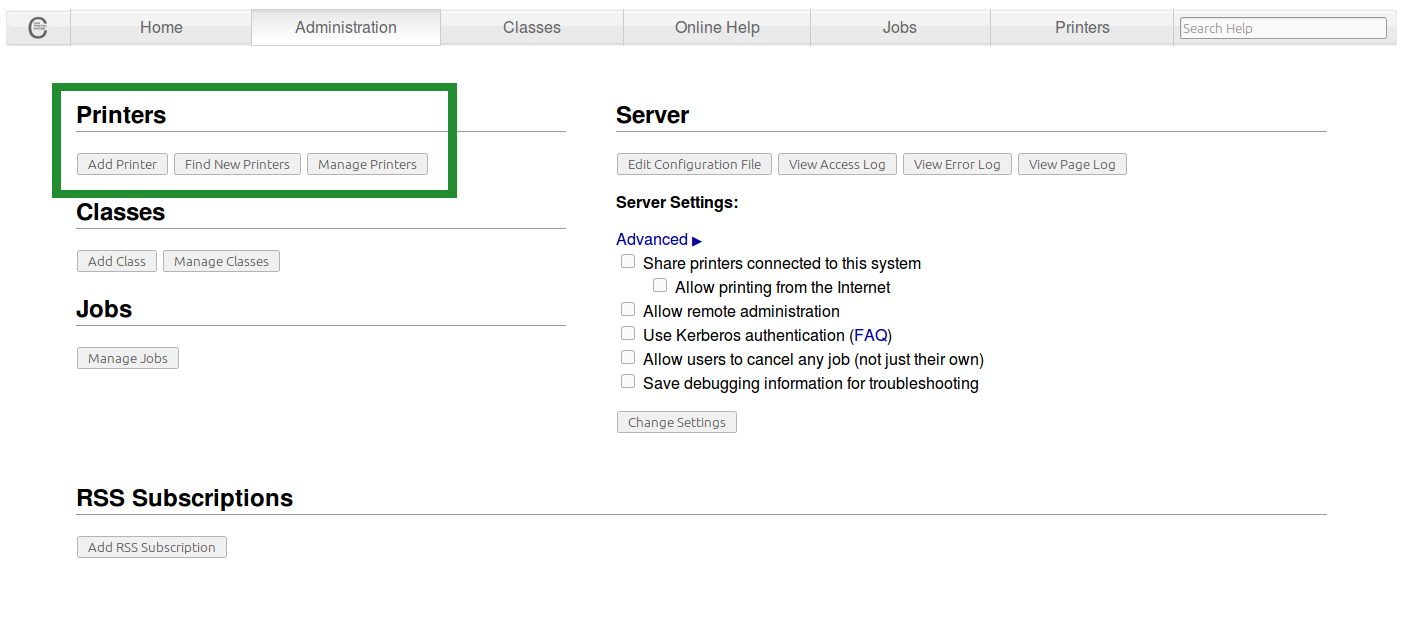
\includegraphics[width=1\textwidth]{imgs/filter-failed-4.png}
  \caption{Adding the printer on the \emph{Administration} page.}
  \label{fig4}
\end{figure}

\noindent Once that is complete, try printing your document. (You can also print a test page in the \emph{Maintenance} menu of your printer's page (Figure~\ref{fig5}).)

\begin{figure}[!hbp]
  \centering
  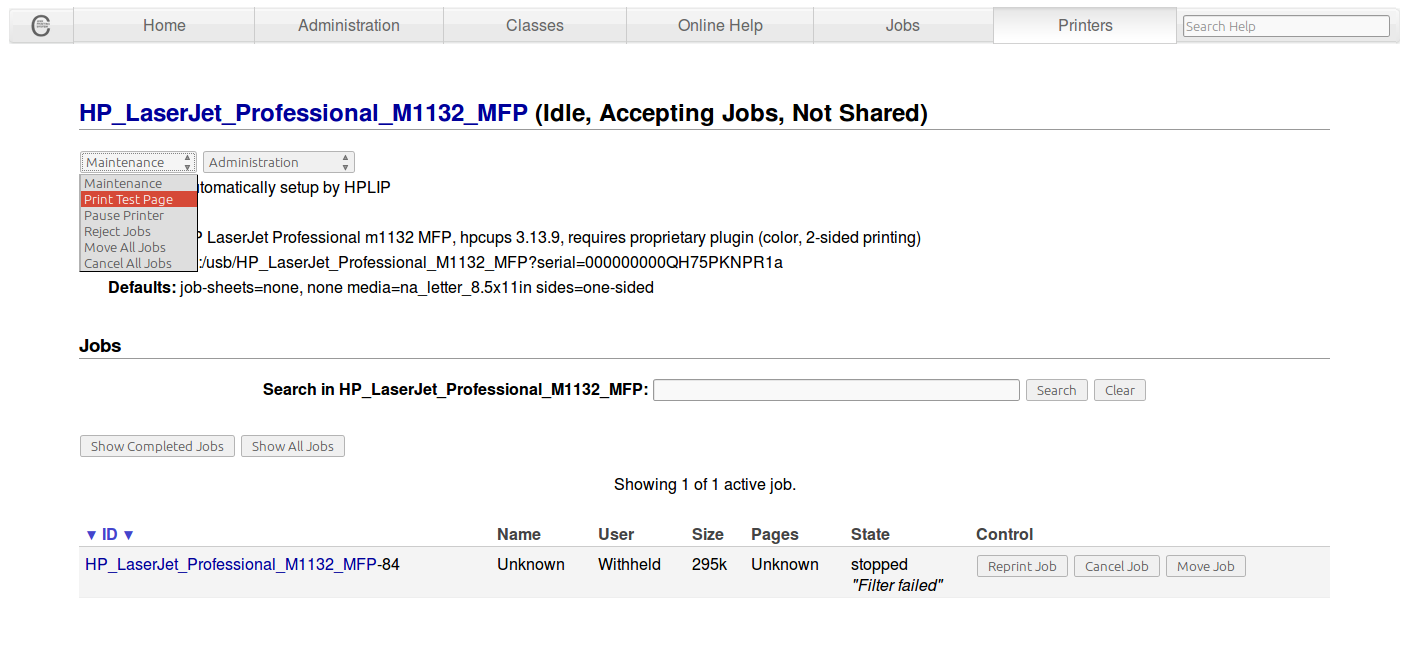
\includegraphics[width=1\textwidth]{imgs/filter-failed-5.png}
  \caption{Printing a test page using the \emph{Maintenance} menu.}
  \label{fig5}
\end{figure}

\noindent Alternate solution if this fails: rename your printer with a slightly different name.

\subsection*{Solution 2: re-install CUPS}\addcontentsline{toc}{subsection}{Solution 2: re-install CUPS}

Some found that this error was caused by a problem with CUPS, either after an update or failed installation.

Although you can do this in the terminal, we're going to use a GUI method. Open Synaptic, and in the \emph{Quick filter} text field, type “cups” (Figure~\ref{fig6}).

\newpage
\begin{figure}[!hbp]
  \centering
  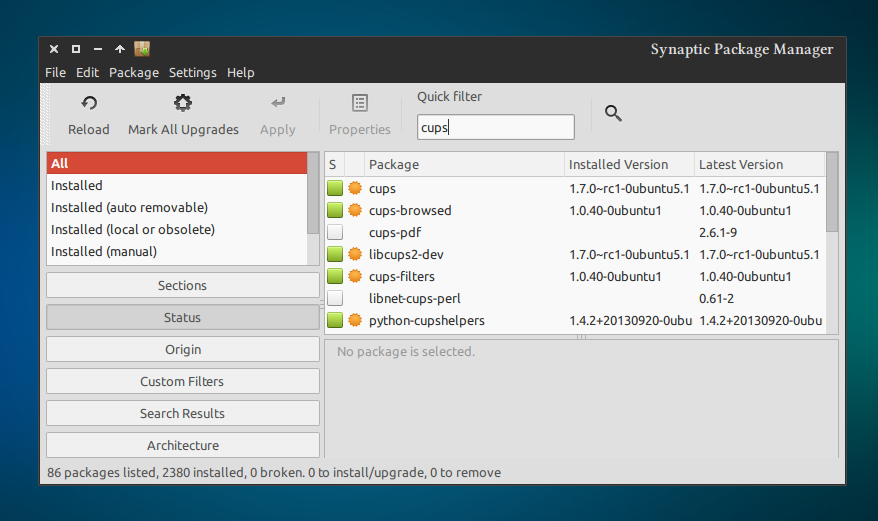
\includegraphics[width=1\textwidth]{imgs/filter-failed-6.png}
  \caption{Finding CUPS in Synaptic.}
  \label{fig6}
\end{figure}

\noindent Click on the \emph{Installed} tab, so it will be easier to select all (Figure~\ref{fig7}). Although you don't have to re-install everything, this is what I (or we) will be doing. 

\begin{figure}[!hbp]
  \centering
  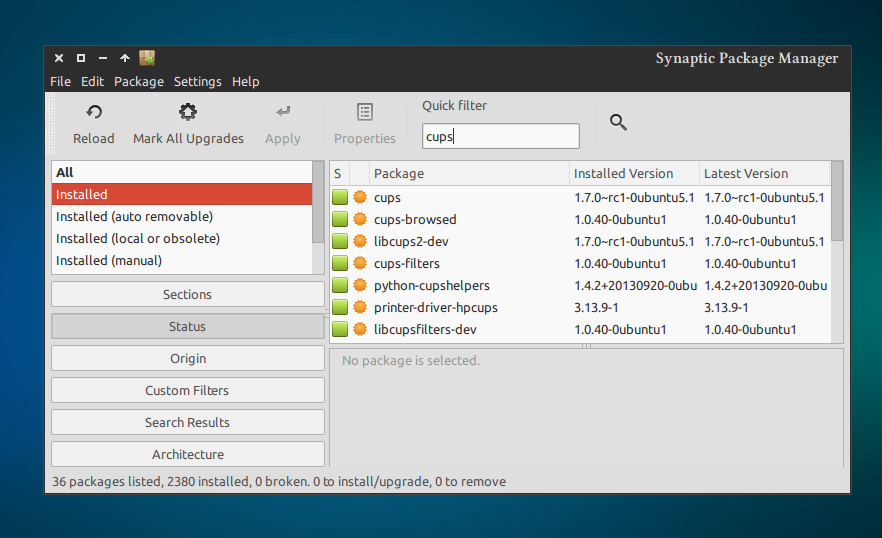
\includegraphics[width=1\textwidth]{imgs/filter-failed-7.png}
  \caption{Viewing all CUPS-related installations.}
  \label{fig7}
\end{figure}

\noindent Select all the packages (CTRL + A). Now mark the packages for re-installation (Figure~\ref{fig8}). You can do this either by right-clicking and clicking \emph{Mark for Reinstallation} or opening the \emph{Package} menu and clicking \emph{Mark for Reinstallation} there.

\begin{figure}[!hbp]
  \centering
  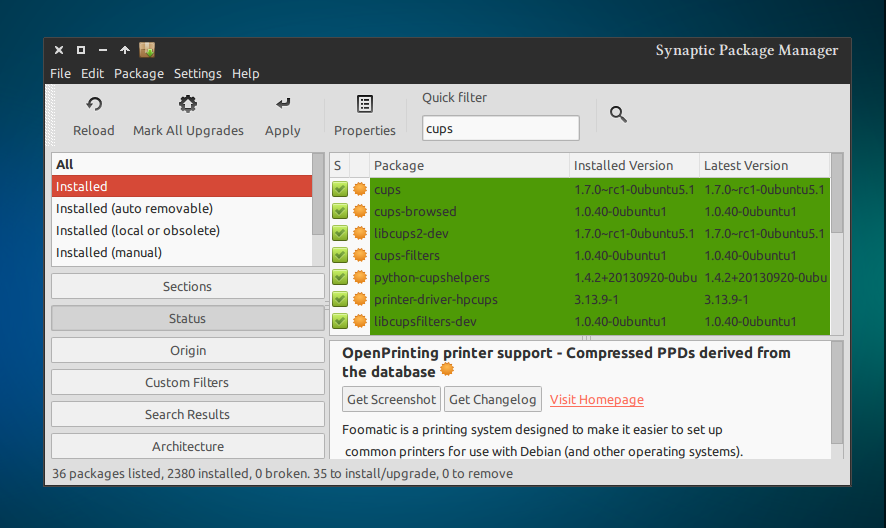
\includegraphics[width=1\textwidth]{imgs/filter-failed-8.png}
  \caption{Marking CUPS for re-installation.}
  \label{fig8}
\end{figure}

\noindent Now click \emph{Apply} and let Synaptic re-install CUPS. After re-installation, print your document.

\subsection*{Solution 3: fix HPLIP}\addcontentsline{toc}{subsection}{Solution 3: fix HPLIP}

\noindent If you perused the list of packages you marked for re-installation, you may have noticed one called hplip. Formally known as HP Linux Imaging and Printing, HPLIP integrates HP printers with Linux. It is provided by HP\footnote{\url{http://hplipopensource.com/hplip-web/index.html}}.

Generally, HPLIP will come pre-installed with your distribution; you can confirm that by typing “hplip” in \emph{Quick filter} again. If it's installed, Synaptic will show it as such.

Let's close Synaptic now and open the terminal. In the terminal, type “hp-check -t”. This will check whether HPLIP is working correctly. Figure~\ref{fig9} shows what I found.

\begin{figure}[!hbp]
  \centering
  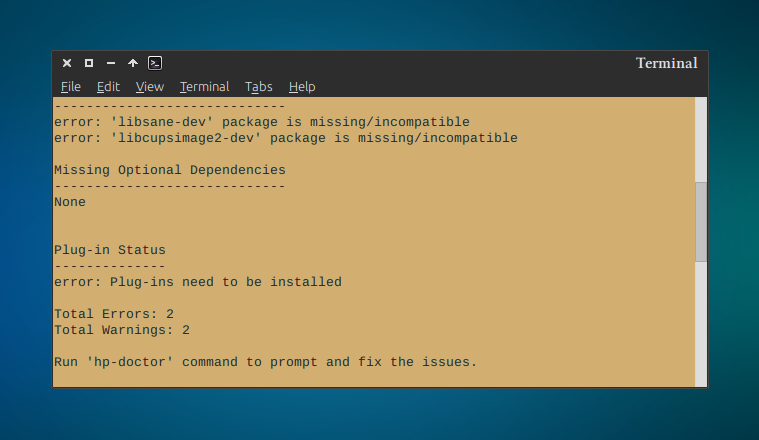
\includegraphics[width=1\textwidth]{imgs/filter-failed-10.png}
  \caption{The results of the ``hp-check -t" command.}
  \label{fig9}
\end{figure}

\noindent I was missing two required packages. If you have the same problem, type “hp-doctor” as suggested. You will get a number of prompts throughout, the first of which may be a distribution error:

\begin{quote}error: This distro (i.e ubuntu 13.10) is either deprecated or not yet supported.\\
The diagnosis is limited on unsupported platforms. Do you want to continue?(y=yes, n=no*):
\end{quote}

\noindent Type “y” and continue. If you get after it checks for updates:

\begin{quote}
Newer version of HPLIP-3.13.11 is available.\\
Press `y' to continue to upgrade HPLIP-3.13.11 (y=yes*, n=no):
\end{quote}

\noindent Type “y” and continue. You may be told to install HPLIP manually, but it will continue anyway, and check for dependencies.

Under \emph{General Dependencies}, hp-doctor found this (Figure~\ref{fig10}):

\newpage
\begin{figure}[!htp]
  \centering
  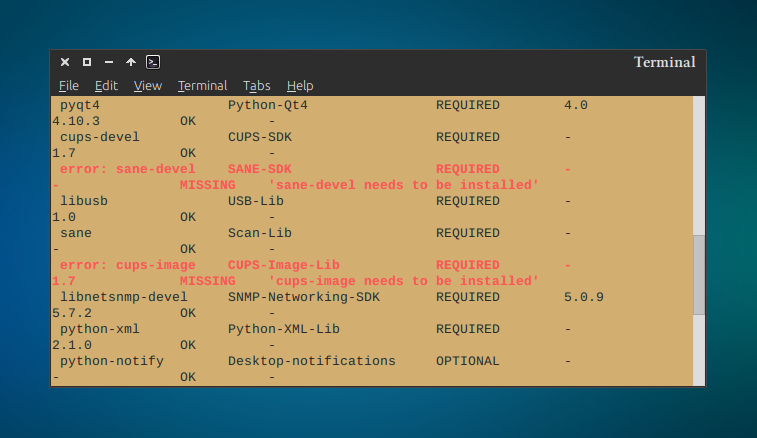
\includegraphics[width=1\textwidth]{imgs/filter-failed-11.png}
  \caption{Running ``hp-doctor" highlights the errors shown by \emph{hp-check -t}. It then attempts to fix them.}
  \label{fig10}
\end{figure}

\noindent The next prompt will be:

\begin{quote}
Do you want to update repository and Install missing/incompatible packages. (a=install all*, c=custom\_install, s=skip):
\end{quote}

\noindent Type “a” and continue. Because my problem was a plug-in version mismatch, I next got this:

\begin{quote}
Found Plugin version mismatch. Press 'y' to re-install the plugin(y=yes*, n=no):
\end{quote}

\noindent Type “y” and continue. When you're asked whether to download, specify a path, or quit, choose the download option by typing “d”.

HP will then ask you to accept the license terms:

\begin{quote}
Do you accept the license terms for the plug-in (y=yes*, n=no, q=quit) ? 
\end{quote}

\noindent Type "y" if you accept. hp-doctor will then complete without further prompts. Now try to print your document.

\subsection*{Other solutions}\addcontentsline{toc}{subsection}{Other solutions}

In my case, running \emph{hp-check -t} was the solution to fix the ``filter failed" error. However, that may not be the case with you.\\

\noindent One solution that was a temporary fix was to change my PDF viewer. So, switching from the default Evince to KDE's Okular\footnote{\url{http://okular.kde.org/}} appeared to solve the problem. (By my own admission, I'm no Linux expert, so don't ask me how.)\\

\noindent Here are some useful resources with other potential solutions:

\begin{itemize}
\item In Arch Linux, one solution is to clean the pacman cache; or install foo2zjs from the AUR while making sure HPLIP is \emph{not} installed: \url{https://bbs.archlinux.org/viewtopic.php?id=148850}.
\item Further advice on using hp-check, et al.: \url{http://unix.stackexchange.com/questions/77139/filter-failed-from-hplip}.
\item If you aren't a member of the lpadmin group, add yourself manually: \url{http://ubuntuforums.org/showthread.php?t=2145030}.
\item Try switching the printer and/or computer off and on again, or trying again later. This solution might seem like a joke, but it's worth a shot if you don't want to re-install packages or play around with the command-line: \url{http://askubuntu.com/questions/304152/after-update-my-printer-will-not-work}.
\end{itemize}

\section*{Error: ``unable to connect to server"}\addcontentsline{toc}{section}{Error: ``unable to connect to server"}

Another error I've discovered is ``unable to connect to server", which has the more serious effect of preventing you from interacting with the printer at all. This means you are unable to load the CUPS interface. When I encountered this error, none of the solutions proposed above worked.

\subsection*{Diagnosing}\addcontentsline{toc}{subsection}{Diagnosing}

Try to open CUPS in your browser, by going to "localhost:631". An error page will come up, stating that the browser is unable to connect to the server at localhost:631 (Figure~\ref{fig11}). Trying to access CUPS using a native printing tool (in my case, system-config-printer\footnote{\url{http://cyberelk.net/tim/software/system-config-printer/}}) initially reports that the "printing service is not available" and gives you the option to connect manually. Doing so, however, brings up the ``failed to connect to server" error.

\begin{figure}[!htp]
  \centering
  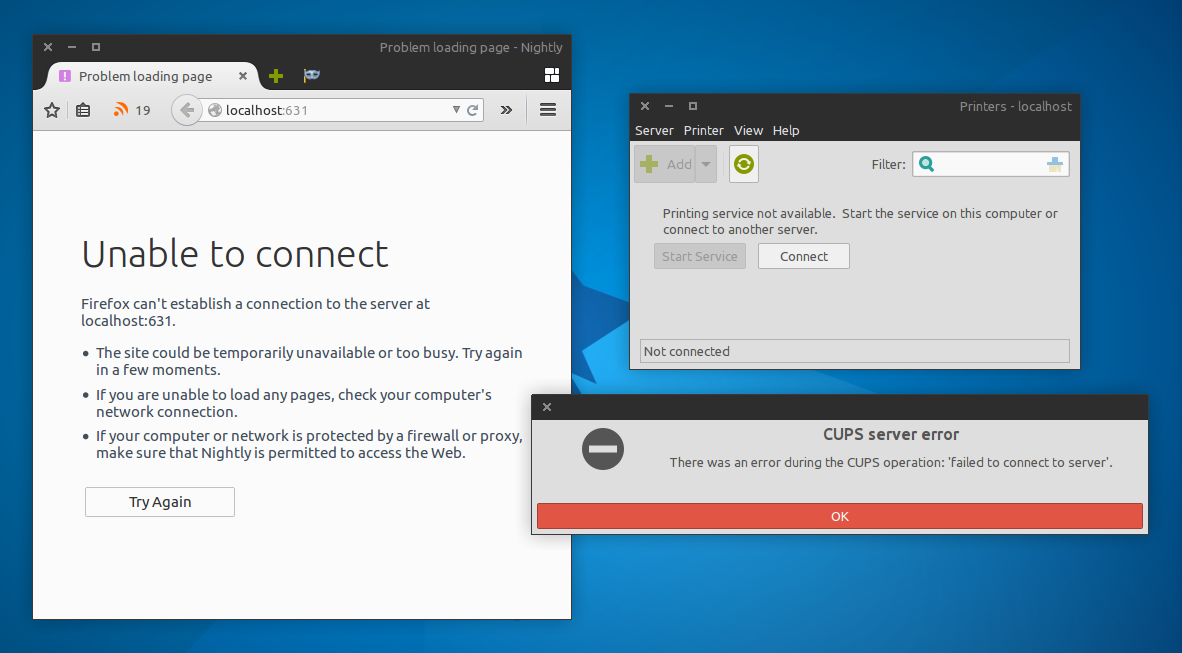
\includegraphics[width=1\textwidth]{imgs/unable-to-connect-to-server-1.png}
  \caption{The ``unable to connect to server" error prevents you from connecting to your printer.}
  \label{fig11}
\end{figure}

\subsection*{Solution 1: edit cupsd.conf}\addcontentsline{toc}{subsection}{Solution 1: edit cupsd.conf}

\emph{\textcolor{Red}{Warning: please be aware that this is solution requires editing a config file in your root directory. If you're worried that this will make the problem worse, either don't try it or do what I do: screenshot every step so you know how to go back and leave the file open so you can always undo the changes after testing.}}\\

\noindent Read the warning? Based on a solution on LinuxQuestions.org.\footnote{\url{https://www.linuxquestions.org/questions/linux-general-1/cups-unable-to-connect-to-server-184088/}},  What we're going to do is edit cupsd.conf to make CUPS listen on port 631. The process is pretty simple---just add the line ``Port 631" or ``Listen 127.0.0.1:631" to cupsd.conf---but for many people, editing 


This solution comes courtesy of a thread 

















\begin{figure}[!htp]
  \centering
  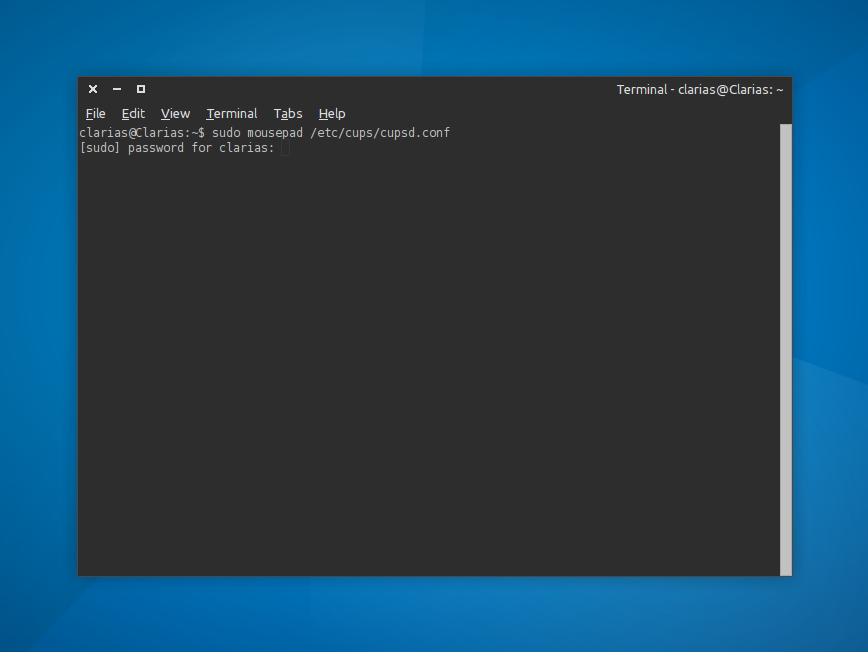
\includegraphics[width=1\textwidth]{imgs/unable-to-connect-to-server-2.png}
  \caption{The ``unable to connect to server" error prevents you from connecting to your printer.}
  \label{fig12}
\end{figure}




\begin{figure}[!htp]
  \centering
  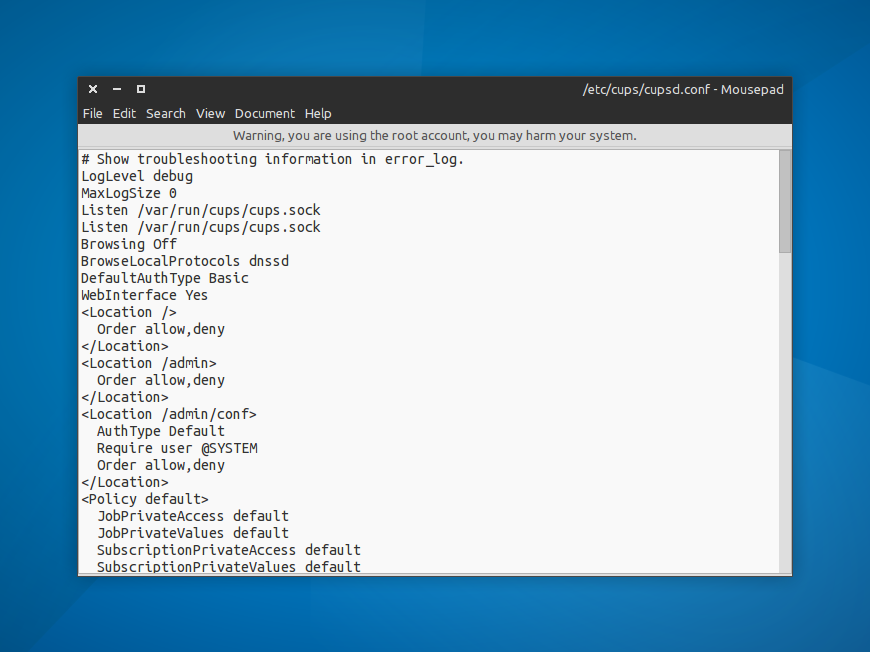
\includegraphics[width=1\textwidth]{imgs/unable-to-connect-to-server-3.png}
  \caption{The ``unable to connect to server" error prevents you from connecting to your printer.}
  \label{fig13}
\end{figure}




\begin{figure}[!htp]
  \centering
  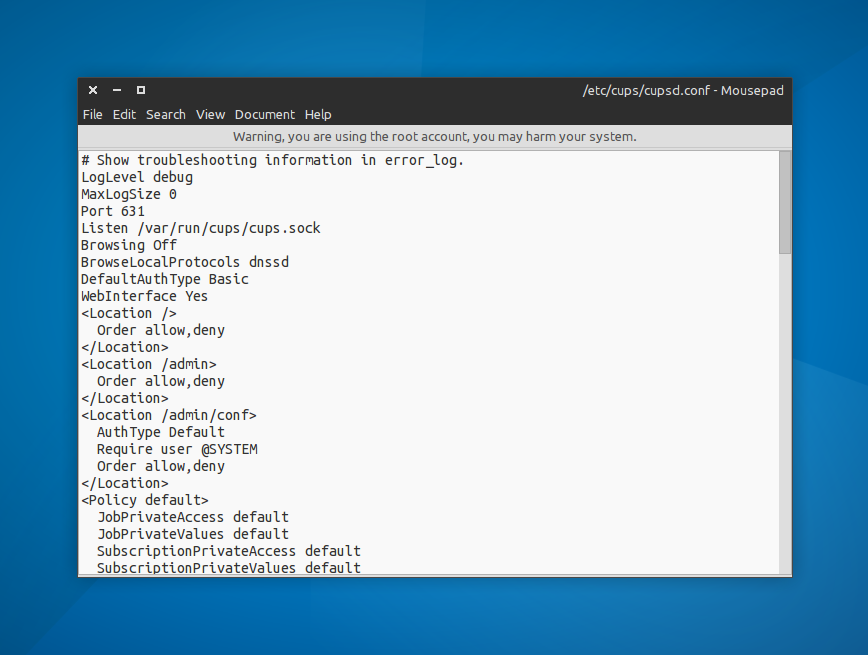
\includegraphics[width=1\textwidth]{imgs/unable-to-connect-to-server-4.png}
  \caption{The ``unable to connect to server" error prevents you from connecting to your printer.}
  \label{fig14}
\end{figure}




\begin{figure}[!htp]
  \centering
  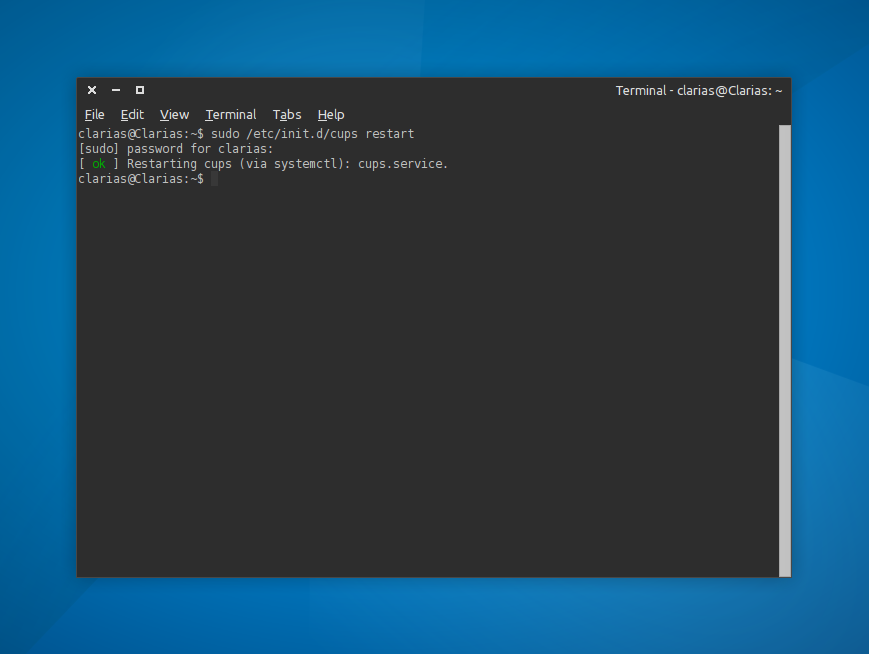
\includegraphics[width=1\textwidth]{imgs/unable-to-connect-to-server-5.png}
  \caption{The ``unable to connect to server" error prevents you from connecting to your printer.}
  \label{fig15}
\end{figure}




\begin{figure}[!htp]
  \centering
  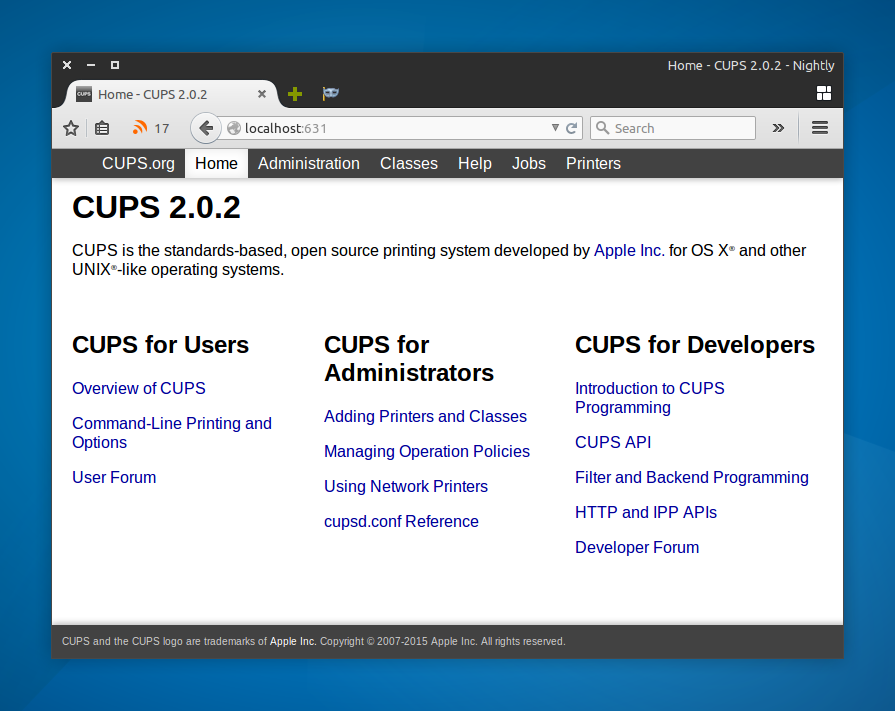
\includegraphics[width=1\textwidth]{imgs/unable-to-connect-to-server-6.png}
  \caption{Success!}
  \label{fig16}
\end{figure}
















This will change how CUPS works, but your computer probably (hopefully) won't explode.








% unable to connect to server

% 1. sudo mousepad /etc/cups/cupsd.conf
% 2. Replace >>> Listen /var/run/cups/cups.sock <<< with >>> Port 631 <<< or >>> Listen 127.0.0.1:631 <<<
% 3. sudo /etc/init.d/cups restart
% 4. hp-doctor

% https://www.linuxquestions.org/questions/linux-general-1/cups-unable-to-connect-to-server-184088/





\vspace{4cm}
\hrule
\noindent \center \emph{Read online at: \url{http://thenumberzero.blogspot.com/2014/02/how-to-fix-hp-printer-filter-failed.html}\\
\textbf{Version} 1.2; \textbf{last edited} 2015-03-02\\
\textbf{License:} Creative Commons Attribution-ShareAlike 4.0 International\\
\textbf{Printer:} HP LaserJet M1132 MFP\\
\textbf{Operating systems tested:} Xubuntu 13.10, 14.04, 14.10; \textbf{theme:} Numix}
\vspace{1em}
\hrule



\end{document}
